\chapter{광자 궤도, 린들러 공간, 슈바르츠실트 내부}

뉴턴 역학의 점질량과 슈바르츠실트 블랙홀은 중력을 만드는 질량이 모두 중심에 집중되어 있다는 동일한 이상화에서 출발한다. 그러나 두 경우에서 중심이 뜻하는 바는 매우 다르다. 뉴턴 역학에서는 각운동량이 아주 조금이라도 있는 입자는 중심을 빗겨 간다. 블랙홀에서는 입자가 지평선을 한 번 넘으면 특이점을 피할 수 없다. 이 차이를 이해하기 위해 원궤도와 광자구를 살펴본 뒤, 지평선 부근의 새로운 좌표계를 알아보겠다.

\section{피할 수 없는 중심}

실제 뉴턴 역학의 물질은 결코 수학적인 점이 되지 않는다. 압력과 물질의 강도, 그 밖의 힘이 압축에 저항한다. 그래도 점질량을 이상화로 사용한다고 하더라도, 낙하하는 입자가 그 질량에 부딪히는 경우는 드물다. 정확히 방사 방향인 궤적은 \(r=0\)에 도달할 수 있지만, 아주 작은 횡방향 속도만 있어도 각운동량이 생긴다. 그러면 원심 장벽이 입자를 중심에서 되돌려 보낸다.

일반상대성이론에서는 결론이 달라진다. 충분히 조밀한 천체는 블랙홀을 형성할 수 있으며, 블랙홀 내부에서는 중심을 돌아 피해 가려는 뉴턴 역학적 탈출이 불가능하다. 그 이유는 단순히 힘이 더 강하기 때문이 아니다. 지평선 안쪽에서는 \(r\)가 감소하는 방향이 미래를 향하는 방향이다. 이 명제는 당연한 전제로 놓기보다 차근차근 도출해 보겠다.

\begin{classroomqa}
\audiencequestion{뉴턴역학에서 중심을 맞히기 어려운 것은 두 물체를 점으로 취급한 데 따른 결과에 불과한가?}
\lecturerresponse{점으로 이상화한 것은 비교의 한 요소이지만 차이의 전부는 아니다. 뉴턴역학에서는 각운동량이 영이 아니기만 하면 궤도가 점을 비껴 지나갈 수 있다. 상대론적 내부에서는 낙하하는 모든 시간꼴 궤적의 미래에 특이점이 놓여 있으므로, 각운동만으로는 벗어날 수 없다.
\lecturetimestamp{00:04:52--00:05:13}}
\end{classroomqa}

\section{지평선과 특이점}

우선 슈바르츠실트 기하를 주어진 것으로 두자.
\begin{equation}
d\tau^{2}
=
\left(1-\frac{2MG}{r}\right)dt^{2}
-
\frac{dr^{2}}{1-\frac{2MG}{r}}
-
r^{2}d\Omega^{2}.
\label{eq:l6-schwarzschild}
\end{equation}
이 계량을 결정하는 장방정식은 나중에 다룬다. 지금 할 일은 계량이 말해 주는 바를 배우는 것이다.

단위구의 계량은 다음과 같이 쓸 수 있다.
\begin{equation}
d\Omega^{2}
=d\vartheta^{2}+\cos^{2}\vartheta\,d\phi^{2}
\label{eq:l6-angular-metric}
\end{equation}
여기서 \(\vartheta\)는 적도면에서 잰 위도이다. 축에서 재는 더 일반적인 극각을 사용하면 코사인 대신 사인이 나타난다. 구면대칭성에 따라 모든 궤도를 하나의 고정된 평면 안에 놓을 수 있으므로, 아래 계산에는 각좌표 하나만 남는다.

\begin{figure}[htbp]
\centering
\includegraphics[width=0.88\textwidth]{lecture_06_figure_01.png}
\caption{곡면 \(r=2MG\)과 슈바르츠실트 시공간을 원통 형태로 나타낸 그림. 중심선은 \(r=0\)이며, 빨간 원통은 슈바르츠실트 좌표계에서의 지평선이다.}
\lectureframe{00:09:45}
\end{figure}

원천에서 멀리 떨어지면 \(2MG/r\)는 작아지고 ~\eqref{eq:l6-schwarzschild}은 구면좌표에서 민코프스키 계량에 가까워진다. 두 반지름이 두드러진다:
\begin{equation}
r=2MG,
\qquad
r=0.
\end{equation}
이 둘을 혼동해서는 안 된다. \(r=2MG\)에서 \(dt^{2}\)의 계수는 영이 되고 \(dr^{2}\)의 계수는 발산한다. 슈바르츠실트 좌표계가 특이해진 것이다. 그곳에서 곡률 자체는 유한하게 유지된다. 반면 \(r=0\)에서는 곡률 불변량이 발산한다. 조석장은 유한한 크기의 물체를 반지름 방향으로 한없이 늘리고 횡방향으로 한없이 압축한다. 이것은 좌표의 결함이 아니라 물리적 특이점이다.

\subsection{낙하 시간을 재는 두 가지 방법}

지평선 바깥에서 정지해 있는 시계의 경우,
\begin{equation}
d\tau
=
\sqrt{1-\frac{2MG}{r}}\,dt.
\label{eq:l6-static-clock}
\end{equation}
\(r\)가 클 때는 \(d\tau\simeq dt\)이다. 지평선에 가까워지면, \(r\)를 고정한 채 유지되는 시계의 고유시간은 멀리 떨어진 곳에서 재는 슈바르츠실트 시간에 비해 매우 느리게 흐른다.

같은 좌표계로 기술하면, 방사 방향 낙하체가 \(r=2MG\)에 도달하는 데 필요한 \(t\)는 무한대가 된다. 그러나 낙하체가 직접 겪는 고유시간은 유한하다. 두 진술은 서로 모순되지 않는다. 낙하체에 실린 시계는 그 세계선을 따라 흐른 고유시간을 잰다. 그것은 기계식 시계일 수도, 미터 막대 양 끝의 거울로 만든 광시계일 수도, 심장 박동일 수도, 뇌에서 일어나는 물리적 과정의 연속일 수도 있다. 어느 것도 멀리 떨어진 좌표 \(t\)를 재지는 않는다. 두 시계의 차이는 지평선 부근의 그림에서 드러날 것이다.

\section{고유시간 작용으로부터 원운동 구하기}

낙하 문제로 돌아가기 전에 다른 문제를 풀어 보자. 질량이 있는 입자나 광자는 어떤 조건에서 블랙홀 주위를 원운동할 수 있을까? 계산은 자유롭게 움직이는 상대론적 입자에 쓰이는 것과 같은 작용 원리에서 출발한다.
\begin{equation}
S=-m\int d\tau.
\label{eq:l6-particle-action}
\end{equation}
빛은 지구에 의해 휘어지지만, 지구의 중력장은 광선을 궤도에 가둘 만큼 강하지 않다. 지구의 슈바르츠실트 반지름은 겨우 센티미터 정도이다. 강한 중력장에 관한 문제가 중요해지려면 지구 전체를 작은 견과류 크기인 대략 그 정도 규모까지 압축해야 한다.

\(c=1\)로 두고 운동을 적도면에 한정한 다음, 다음과 같이 정의하자.
\begin{equation}
F(r)=1-\frac{2MG}{r},
\qquad
G(r)=\frac{1}{F(r)}.
\label{eq:l6-fg}
\end{equation}
좌표시간 \(t\)을 매개변수로 사용하면
\begin{equation}
d\tau
=dt\sqrt{F-G\dot r^{\,2}-r^{2}\dot\theta^{\,2}},
\end{equation}
따라서
\begin{equation}
\mathcal L
=
-m\sqrt{F-G\dot r^{\,2}-r^{2}\dot\theta^{\,2}}.
\label{eq:l6-lagrangian}
\end{equation}
인자 \(m\)는 작용의 차원을 통상적인 에너지 곱하기 시간으로 만들어 준다.

\begin{figure}[htbp]
\centering
\includegraphics[width=0.76\textwidth]{lecture_06_figure_02.png}
\caption{판서에 적고 있는 제곱근 형태의 입자 라그랑지안. 완전한 식은 식~\eqref{eq:l6-lagrangian}에 나와 있다.}
\lectureframe{00:31:53}
\end{figure}

임의의 일반화 좌표 \(q\)에 대해,
\begin{equation}
p_q=\frac{\partial\mathcal L}{\partial\dot q}.
\end{equation}
라그랑지안에는 \(\mathcal L\)를, 각운동량에는 \(L\)를 사용하는 것이 편리하다. 다음과 같이 놓으면
\begin{equation}
\Delta=F-G\dot r^{\,2}-r^{2}\dot\theta^{\,2},
\end{equation}
두 운동량은 다음과 같다.
\begin{align}
L=p_\theta
&=\frac{mr^{2}\dot\theta}{\sqrt{\Delta}},
\label{eq:l6-angular-momentum}\\
p_r
&=\frac{mG\dot r}{\sqrt{\Delta}}.
\label{eq:l6-radial-momentum}
\end{align}
방사 좌표가 라그랑지안에 나타나므로 방사 운동량은 보존되지 않는다. 각도 \(\theta\)는 라그랑지안에 나타나지 않으므로 \(L\)는 보존된다.

또한 \(\mathcal L\)에는 \(t\)가 명시적으로 나타나지 않는다. 따라서 해밀토니안은 보존된다.
\begin{align}
E=H
&=p_r\dot r+L\dot\theta-\mathcal L \\
&=\frac{mG\dot r^{\,2}}{\sqrt{\Delta}}
  +\frac{mr^{2}\dot\theta^{\,2}}{\sqrt{\Delta}}
  +m\sqrt{\Delta} \\
&=\frac{mF}{\sqrt{\Delta}}.
\label{eq:l6-energy-general}
\end{align}
이는 역학에서 되풀이되는 전형적인 흐름이다. 원리로부터 작용이 나오고, 계산을 통해 운동량을 구하며, 대칭성이 계산 결과를 에너지와 각운동량 보존 원리로 연결한다. 오일러--라그랑주 방정식을 곧바로 모두 풀 수도 있지만, 회전 대칭성과 시간 병진 대칭성으로 얻는 상수들을 이용하면 작업을 크게 줄일 수 있다.

\subsection{원궤도의 에너지}

원궤도에서는
\begin{equation}
\dot r=0.
\end{equation}
단위 질량당 각운동량을 다음과 같이 정의하자.
\begin{equation}
\lambda=\frac{L}{m}.
\end{equation}
식~\eqref{eq:l6-angular-momentum}과
\eqref{eq:l6-energy-general}은 다음과 같이 된다.
\begin{align}
\lambda
&=\frac{r^{2}\dot\theta}
{\sqrt{F-r^{2}\dot\theta^{\,2}}},
\label{eq:l6-lambda-circular}\\
E
&=\frac{mF}{\sqrt{F-r^{2}\dot\theta^{\,2}}}.
\label{eq:l6-energy-circular-first}
\end{align}

\begin{figure}[htbp]
\centering
\includegraphics[width=0.82\textwidth]{lecture_06_figure_04.png}
\caption{슈바르츠실트 시공간에서 원운동할 때의 단위 질량당 각운동량과 에너지. 각운동량 식을 먼저 이용해 에너지 식에서 \(\dot\theta\)를 없앤다.}
\lectureframe{00:39:14}
\end{figure}

식~\eqref{eq:l6-lambda-circular}을 제곱하고 각속도를 구하면
\begin{equation}
\dot\theta^{\,2}
=
\frac{\lambda^{2}F}
{r^{2}\left(r^{2}+\lambda^{2}\right)}.
\label{eq:l6-angular-speed}
\end{equation}
이를 식~\eqref{eq:l6-energy-circular-first}에 대입하면, 제안된 반지름과 고정된 각운동량에만 의존하는 에너지가 남는다.
\begin{equation}
E(r,\lambda)
=m\sqrt{F(r)}\,\frac{\sqrt{r^{2}+\lambda^{2}}}{r}.
\label{eq:l6-circular-energy}
\end{equation}

강의에서는 뉴턴 역학과의 비교를 잠시 살펴본다. 일반적인 원궤도에서는 반지름이 커질수록 각진동수와 접선 속력이 감소하지만, 각운동량에는 반지름 인자가 포함된다. 그러므로 각속도만 보고 \(L\)가 어떻게 변하는지 추론해서는 안 된다. 상대론적 식은 이 인자들을 명시적으로 드러낸다.

\section{빛의 원궤도}

광자는 정지 질량이 없는데도 에너지와 운동량을 가진다. 따라서 ~\eqref{eq:l6-circular-energy}의 질량 없는 극한은 주의해서 취해야 한다. \(m\)이 \(\lambda\)를 고정한 채 영으로 가면 \(L=m\lambda\)도 영이 된다. 대신 다음과 같이 극한을 취한다.
\begin{equation}
m\longrightarrow0,
\qquad
\lambda\longrightarrow\infty,
\qquad
L=m\lambda\ \text{fixed}.
\label{eq:l6-massless-limit}
\end{equation}
그러면 \(\lambda^{2}\) 항이 지배적이 되고 광자의 에너지는 다음과 같이 된다.
\begin{equation}
E_\gamma(r;L)
=L\,\frac{\sqrt{1-\frac{2MG}{r}}}{r}.
\label{eq:l6-photon-energy}
\end{equation}
인자 \(L\)는 반지름에 따른 함수 전체에 곱해진다. 이는 에너지 척도에는 영향을 주지만 원궤도의 반지름에는 영향을 주지 않는다.

\begin{figure}[htbp]
\centering
\includegraphics[width=0.88\textwidth]{lecture_06_figure_05.png}
\caption{광자 에너지의 반지름 인자. 지평선에서 영이 되고, 큰 반지름에서는 영을 향해 감소하며, 그 사이에 최댓값이 하나 있다.}
\lectureframe{00:50:50}
\end{figure}

\(L\)를 고정했을 때 방사 방향 평형이 성립하려면 정지점이어야 한다.
\begin{equation}
\frac{d}{dr}
\left[
\frac{\sqrt{1-\frac{2MG}{r}}}{r}
\right]=0.
\end{equation}
미분하면
\begin{equation}
-\frac{\sqrt{1-\frac{2MG}{r}}}{r^{2}}
+
\frac{MG}
{r^{3}\sqrt{1-\frac{2MG}{r}}}
=0,
\end{equation}
따라서
\begin{equation}
r=3MG.
\label{eq:l6-photon-sphere}
\end{equation}
이 반지름은 슈바르츠실트 반지름의 1.5배이다. 보통 이를 광자구라고 부른다.

이 정지점은 최댓값이므로 광자의 원궤도는 불안정하다. 정확히 \(3MG\)에 놓인 광자는 그 자리에 머문다. 방사 방향으로 아주 조금만 벗어나도 결국 최댓값에서 멀어진다. 광자구 바로 바깥에서는 광선이 탈출하기 전에 매우 큰 각도만큼 휩쓸고 지나가 블랙홀 주위를 여러 바퀴 돌 수도 있다. 광자구 바로 안쪽에서는 거의 접선 방향으로 움직이는 광선이 여러 바퀴 돈 뒤 지평선을 통과해 안으로 떨어질 수 있다.

\begin{figure}[htbp]
\centering
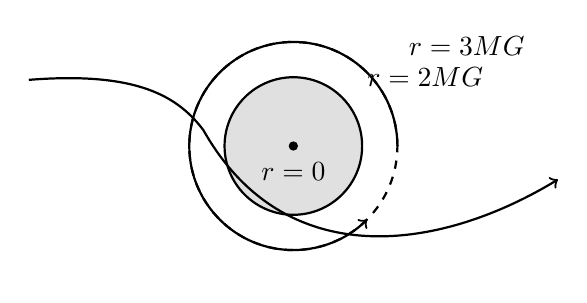
\begin{tikzpicture}[scale=1.12]
\fill[black!12] (0,0) circle (0.78);
\draw[thick] (0,0) circle (0.78);
\draw[dashed,thick] (0,0) circle (1.18);
\fill (0,0) circle (1.5pt);
\draw[->,thick] (1.18,0) arc (0:315:1.18);
\draw[->,thick] (-3.0,0.75)
  .. controls (-1.75,0.85) and (-1.30,0.55) .. (-1.02,0.18)
  .. controls (-0.10,-1.45) and (1.65,-1.20) .. (3.0,-0.38);
\node[right] at (0.73,0.78) {\(r=2MG\)};
\node[right] at (1.20,1.13) {\(r=3MG\)};
\node[below] at (0,-0.08) {\(r=0\)};
\end{tikzpicture}
\caption{지평선, 광자구, 그리고 크게 휘어진 광선. 불안정한 원궤도에 임의로 가까운 광선은 탈출하거나 안쪽으로 떨어지기 전에 임의로 큰 각도만큼 휘어질 수 있다.}
\end{figure}

\begin{classroomqa}
\audiencequestion{각운동량을 고정하는 이유는 무엇이며, 각운동량은 광자의 진동수 및 입사 궤적과 어떤 관계가 있는가?}
\lecturerresponse{모든 광선은 블랙홀을 기준으로 보존되는 각운동량을 가진다. 광자의 진동수는 선운동량의 크기를 정하고, 중심으로부터의 편차는 \(L\)를 정하는 데 기여한다. 원궤도에서 벗어나 있으면 반지름과 각운동량을 독립적으로 정할 수 있다. 광자 원궤도 조건을 요구하면 운동은 유일한 반지름 \(3MG\)와 연결되며, 식~\eqref{eq:l6-photon-energy}의 인수분해를 보면 이 반지름이 \(L\)의 크기와 무관함을 알 수 있다.
\lecturetimestamp{00:54:43--00:57:02}}
\end{classroomqa}

\begin{classroomqa}
\audiencequestion{에너지의 최댓값이 왜 궤도 위치를 정하는가?}
\lecturerresponse{각운동을 제거하고 \(L\)를 고정하면, 남은 함수는 유효 방사 에너지 역할을 한다. 정지점은 방사 방향 평형을 제공한다. 최솟값이라면 안정하지만, 이 점은 최댓값이므로 불안정한 원궤도가 된다. 평형 상태이면서 동시에 불안정하다고 부르는 데에는 모순이 없다.
\lecturetimestamp{00:57:51--00:58:54}}
\end{classroomqa}

질량이 있는 입자는 \(3MG\) 바깥에서 시간꼴 원궤도를 가질 수 있지만, 광자구에 가장 가까운 궤도들은 불안정하다. 질량이 없는 입자는 \(3MG\)에 있는 원궤도만 가질 수 있다. 광자구 안쪽에서 접선 방향으로 움직이는 광자는 안쪽으로 떨어진다. 더 느리게 움직이는 물체라고 해서 그런 궤도를 유지할 가능성이 더 큰 것도 아니다. 이 명제는 각운동에 관한 것이다. 지평선 바깥에서는 시작 반지름이 \(3MG\)보다 작더라도 충분히 바깥쪽을 향하는 광선은 여전히 탈출할 수 있다.

\section{블랙홀이 상에 미치는 영향}

광자구를 생각하면 블랙홀이 그저 변함없는 밤하늘 위에 검은 원반을 붙여 놓은 것이 아님을 알 수 있다. 배경 천체에서 온 빛은 여러 경로를 따라 관측자에게 도달할 수 있다. 한 광선은 블랙홀 한쪽으로 지나고 다른 광선은 반대쪽으로 지나갈 수 있으며, 또 다른 광선들은 블랙홀 주위를 한 바퀴 이상 돌 수도 있다. 그 결과 위치가 어긋난 상, 중복된 상, 고리, 그리고 더 많이 감긴 경로에 해당하는 점점 더 미세하고 어두운 무한한 상의 열이 나타날 수 있다. 정확한 모습은 복잡하지만, 그 원인은 불안정한 궤도에 이미 담겨 있다.

광원과 렌즈, 관측자가 충분히 일직선에 놓이면 상이 아인슈타인 고리를 이룰 수 있다. 중력렌즈에 의한 고리는 자연에서 관측된다. 블랙홀의 상을 완전히 계산하려면 여러 초기 방향에서 시작하는 빛꼴 측지선을 적분해야 하며, 컴퓨터를 이용하기에 적합한 계산이다.

\begin{classroomqa}
\audiencequestion{이 광학적 경계는 광자구를 가리키는가, 지평선을 가리키는가?}
\lecturerresponse{두 경계의 역할은 서로 다르다. \(2MG\)에 있는 지평선은 인과적 경계로, 그 안에서 미래 방향으로 향하는 신호는 밖으로 탈출할 수 없다. \(3MG\)에 있는 광자구는 접선 방향 운동과 강한 중력렌즈 효과를 좌우한다. 두 반지름 사이에서는 바깥쪽 방사 광선이 탈출할 수 있지만, 접선 방향 광선은 안으로 떨어진다. 중간 방향의 광선은 탈출하거나 포획되기 전에 몇 바퀴 돌 수도 있다.
\lecturetimestamp{01:02:47--01:03:40}}
\end{classroomqa}

\begin{classroomqa}
\audiencequestion{일반적인 빛의 경로를 개략적으로 그리는 데 그치지 않고 계산할 수 있는가?}
\lecturerresponse{그렇다. 빛꼴 조건을 측지선 방정식이나 오일러--라그랑주 방정식에 대입한 다음, 선택한 초기 조건으로 적분하면 된다. 개념적으로 새로운 방정식은 아니지만 광선 추적은 대수적으로 복잡하기 때문에, 실제 상을 구할 때는 수치 계산이 실용적인 방법이다.
\lecturetimestamp{01:03:48--01:04:27}}
\end{classroomqa}

\begin{classroomqa}
\audiencequestion{오일러--라그랑주 방정식을 바로 적용했다면 원궤도 계산이 더 어려워졌을까?}
\lecturerresponse{같은 결과를 얻었을 것이다. 어느 방법에서든 작용이 올바른 출발점이지만, 순환 좌표를 이용하면 보존되는 에너지와 각운동량을 알아낼 수 있다. 이 상수들을 먼저 이용하는 것이 원궤도 조건을 구하는 더 짧은 길이다.
\lecturetimestamp{01:04:33--01:05:49}}
\end{classroomqa}

\section{지평선 부근의 계량은 린들러 공간}

이제 지평선으로 돌아가자. 슈바르츠실트 계수들은 지평선에서 발산하거나 영이 되는 듯 보이며, 지평선을 통과하면 부호가 서로 바뀐다. 그런데도 낙하하는 관측자는 그 표면에서 국소 곡률이 발산하는 일을 겪지 않는다. 등가원리는 이 두 진술이 어떻게 동시에 참일 수 있는지 알려준다.

2차원 민코프스키 시공간에서 시작하자.
\begin{equation}
d\tau^{2}=dT^{2}-dX^{2}.
\end{equation}
오른쪽 린들러 쐐기에서 다음과 같이 정의하자.
\begin{equation}
X=\rho\cosh\omega,
\qquad
T=\rho\sinh\omega.
\label{eq:l6-rindler-map}
\end{equation}
\(\rho\)가 일정한 곡선은 다음을 만족한다.
\begin{equation}
X^{2}-T^{2}=\rho^{2},
\end{equation}
따라서 이들은 쌍곡선이며, 균일하게 가속하는 관측자의 세계선이다. 식~\eqref{eq:l6-rindler-map}를 평탄한 계량에 대입하면
\begin{equation}
d\tau^{2}
=\rho^{2}d\omega^{2}-d\rho^{2}.
\label{eq:l6-rindler-metric}
\end{equation}
이제 다음과 같이 놓자.
\begin{equation}
\rho^{2}=4\xi,
\qquad
\omega=\frac{t}{2}.
\label{eq:l6-rindler-rescale}
\end{equation}
\(d\rho^{2}=d\xi^{2}/\xi\)이므로 식~\eqref{eq:l6-rindler-metric}은 다음과 같이 된다.
\begin{equation}
d\tau^{2}
=\xi\,dt^{2}-\frac{d\xi^{2}}{\xi}.
\label{eq:l6-xi-metric}
\end{equation}

\begin{classroomqa}
\audiencequestion{각좌표나 횡방향 좌표는 어디로 갔는가?}
\lecturerresponse{생략했을 뿐이다. 지평선 통과 거동을 포함하는 국소 \(t\)-\(r\) 평면을 살펴보고 있다. 두 횡방향은 여전히 정칙이며 다시 포함할 수 있다. 이들은 지금 분석하는 좌표 특이점에 영향을 주지 않는다.
\lecturetimestamp{01:16:27--01:16:47}}
\end{classroomqa}

슈바르츠실트 계량과 비교하기 위해 \(2MG=1\)인 단위계를 택하자. 식~\eqref{eq:l6-schwarzschild}의 방사 방향 부분은
\begin{equation}
d\tau^{2}
=
\frac{r-1}{r}\,dt^{2}
-
\frac{r}{r-1}\,dr^{2}.
\end{equation}
\(r=1\)에 아주 가까우면 작은 분자 \(r-1\)는 남겨 두어야 하지만, 그 밖에 큰 영향을 주지 않는 \(r\) 인자들은 1로 바꾸어도 된다. 따라서
\begin{equation}
d\tau^{2}
\simeq
(r-1)\,dt^{2}
-
\frac{dr^{2}}{r-1}.
\end{equation}
다음과 같이 놓으면
\begin{equation}
\xi=r-1,
\end{equation}
이는 정확히 식~\eqref{eq:l6-xi-metric}이다. 지평선 부근의 슈바르츠실트 기하는 평탄한 시공간을 린들러 좌표로 기술한 것과 국소적으로 같다.

\begin{classroomqa}
\audiencequestion{바탕이 되는 시공간이 평탄한데 어떻게 가속 좌표계일 수 있는가?}
\lecturerresponse{가속은 관측자의 성질이지, 반드시 곡률의 성질인 것은 아니다. \(\rho\)를 고정한 세계선은 민코프스키 시공간에서 균일하게 가속한다. 마찬가지로 블랙홀 가까이에서 반지름을 고정한 채 버티려면 자유낙하를 막아 줄 지지가 필요하다. 전체 슈바르츠실트 시공간은 곡률을 가지지만, 등가원리에 따라 국소적인 기술은 서로 일치한다.
\lecturetimestamp{01:22:19--01:24:06}}
\end{classroomqa}

\section{린들러 지평선 통과}

오른쪽 쐐기의 공식은 \(\xi>0\)인 영역만을 다룬다.
\begin{equation}
X=2\sqrt{\xi}\cosh\frac{t}{2},
\qquad
T=2\sqrt{\xi}\sinh\frac{t}{2}.
\label{eq:l6-rindler-outside}
\end{equation}
면 \(\xi=0\)는 영선 \(X=T\)이다. 미래 쐐기 안쪽으로 이어 가려면 다음과 같이 놓고
\begin{equation}
\zeta=-\xi>0
\end{equation}
쌍곡함수의 역할을 서로 바꾸자.
\begin{equation}
T=2\sqrt{\zeta}\cosh\frac{t}{2},
\qquad
X=2\sqrt{\zeta}\sinh\frac{t}{2}.
\label{eq:l6-rindler-inside}
\end{equation}
계량은 여전히 다음과 같다.
\begin{equation}
d\tau^{2}
=\xi\,dt^{2}-\frac{d\xi^{2}}{\xi},
\end{equation}
그러나 \(\xi<0\)이면 \(dt^{2}\)의 계수는 음수이고 \(d\xi^{2}\)의 계수는 양수이다. 좌표 \(\xi\), 따라서 슈바르츠실트의 방사 방향은 시간꼴이 되었고, \(t\)는 공간꼴이 되었다.

\begin{figure}[htbp]
\centering
\includegraphics[width=0.88\textwidth]{lecture_06_figure_06.png}
\caption{린들러 쐐기와 영 경계, 그리고 \(\xi>0\)에서 \(\xi<0\)로 이어지는 과정. 칠판에는 \(\rho^{2}=4\xi\)와 \(\omega=t/2\)도 적혀 있다.}
\lectureframe{01:29:40}
\end{figure}

\begin{classroomqa}
\audiencequestion{이 좌표 그림에서 빛보다 빠르게 움직이는 곡선도 있는가?}
\lecturerresponse{좌표 격자선이 물질적 물체의 세계선일 필요는 없다. 좌표상의 기울기가 빛보다 빠른 것처럼 보여도 인과율을 위반하지 않는다. 물리적인 빛은 계속 영선을 따라가고, 물리적인 입자는 계속 국소 광원뿔 내부에 머문다.
\lecturetimestamp{01:28:44--01:29:08}}
\end{classroomqa}

슈바르츠실트 내부를 더 들어가면 결국 \(r=0\)에 이른다. 그 경계는 공간꼴이다. 따라서 이를 장소라기보다 시간으로 설명하는 편이 낫다. 블랙홀 내부의 미래 방향 시간꼴 궤적이나 영꼴 궤적은 모두 그 경계에 도달한다. 장소는 돌아갈 수 있지만, 자신의 미래를 돌아갈 수는 없다.

\begin{classroomqa}
\audiencequestion{\(r=0\)를 통과해 음의 \(r\) 쪽으로 그림을 계속 이어 갈 수 있는가? 그리고 \(r=0\)는 여전히 중심인가?}
\lecturerresponse{좌표 그림에서는 선을 연장하고 싶을 수 있지만, 고전적인 슈바르츠실트 해는 곡률 특이점에서 끝난다. \(r=0\)를 여전히 중심이라고 부를 수는 있지만, 아주 특이한 중심이다. 내부에서 그곳은 공간꼴 미래 경계이다. 음의 반지름 영역으로 이어지는 정칙한 통로는 없다.
\lecturetimestamp{01:32:16--01:34:06}}
\end{classroomqa}

\begin{classroomqa}
\audiencequestion{린들러 그림의 대각선 축들은 빛꼴인가? 낙하체는 가속 시간의 유한한 값에서 그 안으로 들어갈 수 있는가?}
\lecturerresponse{그렇다. 쐐기의 경계는 영선이다. 자유낙하 세계선은 보통의 유한한 사건에서, 그리고 유한한 고유시간 안에 그 선을 통과한다. 가속 좌표 \(t\), 즉 \(\omega\)는 외부의 일정한 \(\rho\) 기술을 따라 무한히 커진다. 무한대가 되는 것은 통과 사건이 아니라 좌표를 부여하는 방식이다.
\lecturetimestamp{01:34:26--01:35:03}}
\end{classroomqa}

\section{바깥의 앨리스와 낙하하는 밥}

앨리스는 중력을 버티도록 지지받으며 일정한 반지름에 머물고, 밥은 자유낙하한다고 하자. 지평선 부근에서 앨리스는 린들러 좌표의 쌍곡선과 비슷한 궤적을 따른다. 앨리스의 일정한 \(t\) 단면은 영 경계에 점점 가까워진다. 앨리스가 유한한 \(t\)로 표시하는 밥의 세계선상 사건은 모두 지평선 바깥에 있다. 따라서 밥이 지평선을 통과하는 순간에 유한한 슈바르츠실트 시간을 부여하는 일은 없다.

밥은 고유시간 시계를 가지고 있다. 밥의 궤적은 그 시계의 유한한 시간 간격 안에 영선을 가로지른다. 통과할 때 국소적으로 발산하는 현상은 일어나지 않는다. 지평선은 전역적으로 결정적인 경계이지만 국소적으로는 평범하다.

\begin{figure}[htbp]
\centering
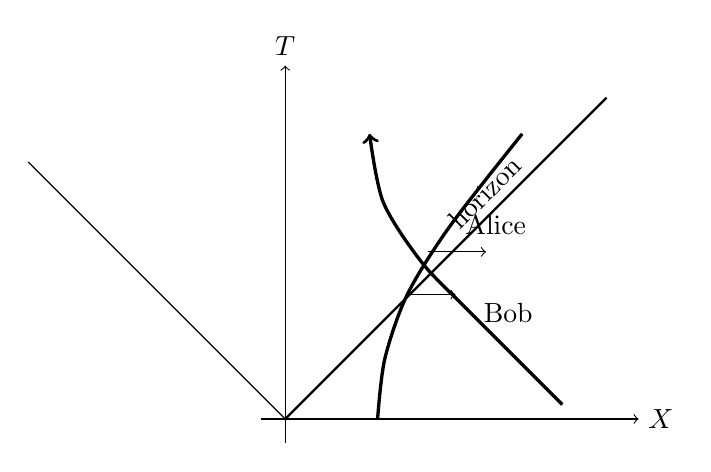
\begin{tikzpicture}[scale=1.02]
\draw[->] (-0.3,0) -- (4.4,0) node[right] {\(X\)};
\draw[->] (0,-0.3) -- (0,4.4) node[above] {\(T\)};
\draw[thick] (0,0) -- (4.0,4.0);
\draw[thin] (0,0) -- (-3.2,3.2);
\node[rotate=45,above] at (2.65,2.65) {horizon};
\draw[very thick]
  plot[smooth] coordinates {(1.15,0.0) (1.24,0.75) (1.52,1.55)
  (2.05,2.40) (2.95,3.55)};
\node[right] at (2.12,2.42) {Alice};
\draw[very thick,->]
  plot[smooth] coordinates {(3.45,0.18) (2.85,0.78) (2.25,1.38)
  (1.70,1.95) (1.22,2.70) (1.05,3.55)};
\node[right] at (2.35,1.32) {Bob};
\draw[->] (1.52,1.55) -- (2.12,1.55);
\draw[->] (1.78,2.08) -- (2.50,2.08);
\end{tikzpicture}
\caption{앨리스의 가속된 외부 세계선과 밥의 자유낙하 세계선. 앨리스의 좌표 단면은 지평선에 가까워지고, 밥은 유한한 고유시간 안에 지평선을 통과한다.}
\end{figure}

\begin{classroomqa}
\audiencequestion{밥이 뒤돌아보면 앨리스는 어떻게 보이며, 밥의 시계는 지평선을 통과한 뒤 어떻게 되는가?}
\lecturerresponse{밥은 앨리스가 바깥에 머물기 위해 필요한 가속을 하며 멀어지는 모습을 보지만, 자신이 지평선을 통과할 때 특이한 사건을 보지는 않는다. 앨리스는 일정한 반지름에 지지된 채 있을 수 있고, 궤도 운동은 별도로 생각할 수 있는 상황이다. 밥의 시계는 계속해서 고유시간 \(\tau\)를 정상적으로 잰다. 내부에서 방사 좌표가 시간꼴이라고 하는 것은 인과 구조를 설명하는 말이다. 밥의 손목시계가 문자 그대로 미터 막대로 변한다는 뜻은 아니다. 밥의 세계선은 결국 \(r=0\)에서 끝난다.
\lecturetimestamp{01:39:51--01:44:45}}
\end{classroomqa}

이제 영선은 단순히 좌표 계수가 이상해지는 한 점이 아니라 지평선 자체임을 알 수 있다. 그 바깥에서는 방사 방향 광선 한 갈래가 바깥으로 움직인다. 그 안에서는 미래 광원뿔의 두 방향 모두 더 작은 \(r\)를 향한다. 모든 미래 방향의 질량 있는 궤적은 이 두 영방향 사이에 머물러야 하므로 특이점에 도달한다.

\section{신호, 적색편이, 그리고 형성되는 지평선}

붕괴하는 물질이 규칙적인 간격으로 빛 펄스를 방출한다고 하자. 먼 곳의 관측자는 뒤이어 오는 펄스를 점점 더 긴 간격을 두고 받는다. 펄스의 주파수는 광학 영역에서 적외선, 마이크로파, 전파로 이동하고 파장은 더욱 길어진다. 이상화된 고전적 계산에서는 외부 관측자가 지평선에 접근하는 물질에서 오는 신호를 계속해서 더 늦게까지 관측할 수 있지만, 실제로는 광원이 빠르게 적색편이되고 어두워져 감지할 수 없게 된다.

\begin{classroomqa}
\audiencequestion{붕괴하는 동안 외부 관측자에게 모든 물질이 지평선에서 그대로 얼어붙은 것처럼 보이는가?}
\lecturerresponse{슈바르츠실트 시간으로 보면 붕괴하는 물질의 표면은 점근적으로 지평선에 다가가며 점점 더 얼어붙은 것처럼 보인다. 실제로 관측되는 것은 빛 신호에 담겨 있고, 그 신호는 점점 더 지연되고 적색편이되며 희미해진다. 이러한 좌표상의 설명은 낙하하는 물질이 무한한 고유시간을 겪는다는 뜻이 아니다.
\lecturetimestamp{01:47:06--01:48:11}}
\end{classroomqa}

\begin{classroomqa}
\audiencequestion{충분히 늦게 관측하면 낙하의 전체 역사를 복원할 수 있는가?}
\lecturerresponse{관측자에게 도달하는 데 성공한 방출 신호를 통해서만 가능하다. 연속된 펄스의 간격은 점점 벌어지고 적색편이는 커진다. 감도가 무한한 이상적 관측자라면 고전적인 신호를 점점 더 긴 파장까지 추적할 수 있겠지만, 실제 관측자에게는 천체가 희미해지며 사라진다.
\lecturetimestamp{01:48:13--01:52:00}}
\end{classroomqa}

\begin{classroomqa}
\audiencequestion{특이점이 장소가 아니라 시간이라고 말할 때 정확히 무슨 뜻인가?}
\lecturerresponse{면은 공간꼴이다. 지평선 안으로 들어가면 미래 방향 시간꼴 곡선이나 영꼴 곡선은 모두 그곳에서 끝난다. 다른 길을 택하면 공간상의 위치를 피할 수 있지만, 미래 방향 세계선을 계속 따라가는 한 미래 경계는 피할 수 없다.
\(r=0\)
\lecturetimestamp{01:52:02--01:53:10}}
\end{classroomqa}

그렇다면 외부 관측자는 물질이 지평선을 통과하는 것을 보지 못하는데 블랙홀은 어떻게 형성되거나 질량이 증가할 수 있을까? 붕괴하는 구형 껍질을 생각해 보자. 전역적 지평선은 미리 존재하는 물질 표면처럼 한 반지름에 고정되어 기다리는 것이 아니다. 지평선은 중심에서 시작해 바깥으로 자라며, 블랙홀 영역이 형성되는 동안 붕괴하는 껍질과 만난다. 외부의 슈바르츠실트 기술에서는 여전히 껍질이 최종 지평선에 점근적으로 다가간다. 지평선이 전역적으로 어떻게 정해지는지를 포함한 완전한 시공간 그림은 다음 강의에서 다룬다.

\begin{figure}[htbp]
\centering
\includegraphics[width=0.90\textwidth]{lecture_06_figure_07.png}
\caption{붕괴하는 껍질과, 중심에서 바깥으로 자라나 껍질과 만나는 지평선. 이 그림은 다음 강의에서 전개할 전역적 붕괴 기하를 미리 보여 준다.}
\lectureframe{01:57:25}
\end{figure}

\begin{classroomqa}
\audiencequestion{외부 좌표 시간으로는 아무것도 지평선을 통과하지 않는데 블랙홀은 어떻게 형성되거나 성장할 수 있는가?}
\lecturerresponse{전제에서 좌표에 관한 진술과 전역적인 진술을 뒤섞고 있다. 붕괴하는 물질은 유한한 고유시간 안에 해당 영역에 도달하지만, 사건지평선은 시공간 전체의 인과 구조로 결정된다. 껍질 그림에서는 지평선이 중심에서 시작해 바깥으로 자라나 껍질과 만난다. 외부 관측자가 지연되고 적색편이된 모습으로 보는 것 역시 그러한 전역적 지평선과 양립한다.
\lecturetimestamp{01:53:11--01:57:34}}
\end{classroomqa}

\section{두 구면 사이의 탈출 방향}

지평선과 광자구는 광선 문제를 서로 다른 경우로 나눈다. 반지름이
\begin{equation}
2MG<r<3MG,
\end{equation}
일 때, 방사 방향 바깥쪽으로 나아가는 광선은 무한대까지 탈출할 수 있다. 접선 방향 광선은 탈출할 수 없으며 안쪽으로 떨어진다. 두 방향 사이에는 탈출 원뿔이 있다. 지평선에 가까워질수록 이 원뿔은 바깥쪽 방사 방향을 중심으로 좁아진다. 지평선을 통과하면 원뿔은 완전히 닫힌다.

\begin{classroomqa}
\audiencequestion{지평선과 광자구 사이에 있는 광원도 신호를 바깥으로 보낼 수 있는가?}
\lecturerresponse{그렇다. 방출 사건이 \(2MG\) 바깥에 있기만 하면 충분히 방사 방향에 가까운 바깥쪽 영선은 탈출한다. \(3MG\) 안쪽에서 각운동을 하는 광선이 안으로 떨어진다는 말은 방사 방향 탈출이 불가능하다는 뜻이 아니다. 결과는 방출 방향에 따라 달라지며, 광원이 지평선에 가까워질수록 허용되는 바깥쪽 방향의 원뿔이 좁아진다.
\lecturetimestamp{01:57:34--01:59:48}}
\end{classroomqa}

\begin{classroomqa}
\audiencequestion{바깥에서 들어온 광선이 광자구 안으로 들어가 방향을 틀고 다시 나올 수 있는가?}
\lecturerresponse{여기서 논하는 종류의 영측지선을 따라서는 불가능하다. 되돌아가는 점에서는 방사 속도가 0이어야 하므로, 그 순간 광선은 \(3MG\)보다 작은 반지름에서 접선 방향을 향해야 한다. 그러나 그곳에서는 각운동 궤적이 되돌아 바깥으로 나오는 대신 안쪽으로 떨어진다. 그래도 두 구면 사이에 이미 있는 광원은 지평선을 통과하기 전에 충분히 방사 방향에 가까운 바깥쪽 광선을 방출할 수 있다.
\lecturetimestamp{01:59:49--02:01:27}}
\end{classroomqa}

마지막 질문은 의도적으로 결론을 내리지 않은 채 남겨 둔다. 앨리스와 밥이 지평선 바깥의 같은 반지름에 매달려 있다고 하자. 서로 가까운 관측자들은 분명 신호를 주고받을 수 있다. 구면을 따라 서로 멀리 떨어져 있다면 직접적인 빛꼴 경로와 그 경로가 허용하는 각도 범위를 명시적으로 측지선 계산을 통해 구해야 한다. 수업에서는 간접 경로를 제안한다. 메시지를 거의 반지름 방향으로 바깥쪽에 있는 더 안전한 반지름의 중계점까지 보낸 뒤 그곳에서 전달하고, 다시 안쪽으로 보낸다. 다른 방법으로는 바깥쪽으로 던진 물체나 신호가 되돌아오게 할 수 있다. 이러한 경로들은 접선 방향의 원궤도가 불가능하다는 사실만으로 바깥쪽 관측자들 사이의 모든 통신이 금지되는 것은 아님을 보여준다.

\begin{classroomqa}
\audiencequestion{지평선 가까이의 같은 반지름에 매달린 두 관측자는 블랙홀을 돌아 서로 통신할 수 있는가?}
\lecturerresponse{국소적으로는 가능하다. 서로 멀리 떨어져 있거나 정반대 위치에 있는 관측자들의 경우, 강의에서는 직접 경로의 한계를 계산하지 않았으므로 이를 정리로 내세워서는 안 된다. 논의에서는 먼저 그 각방향 측지선 문제를 미결로 남겨 둔 다음, 간접 신호는 거의 반지름 방향으로 바깥쪽으로 나아가 더 큰 반지름에서 중계된 뒤 되돌아올 수 있다고 설명한다. 지평선에 가까워질수록 직접 신호를 보낼 수 있는 각도 범위는 점점 좁아지지만, 지평선 바깥에서는 바깥쪽 경로를 이용할 수 있다.
\lecturetimestamp{02:01:29--02:04:17}}
\end{classroomqa}

다음 단계에서는 지평선 부근에 대한 이러한 개략적 설명을 붕괴하는 물체의 전역 기하로 바꾸고, 사건의 지평선이 정확히 어떻게 성장하는지 살펴본다.